\documentclass[
	%parspace, % Add vertical space between paragraphs
	%noindent, % No indentation of first lines in each paragraph
	%nohyp, % No hyphenation of words
	%twoside, % Double sided format
	%draft, % Quicker draft compilation without rendering images
	%final, % Set final to hide todos
]{elteikthesis}[2022/04/30]

% The minted package is also supported for source highlighting
% See minted-intregration.tex for example
\usepackage[newfloat]{minted}

% Document's metadata
\title{Java bytecode interpreter Javában} % title
\date{2023} % year of defense

% Author's metadata
\author{Balázs Zoltán}
\degree{programtervező informatikus BSc}

% Superivsor(s)' metadata
\supervisor{Kozsik Tamás Dr.} % internal supervisor's name
\affiliation{egyetemi docens} % internal supervisor's affiliation

% University's metadata
\university{Eötvös Loránd Tudományegyetem} % university's name
\faculty{Informatikai Kar} % faculty's name
\department{Programozási nyelvek és Fordítóprogramok\\ Tanszék} % department's name
\city{Budapest} % city
\logo{elte_cimer_szines} % logo

% Add bibliography file
\addbibresource{elteikthesis.bib}

% The document
\begin{document}

% Set document language
\documentlang{hungarian}

% List of todos (not in the final document)
%\listoftodos[\todolabel]

\definecolor{Java}{RGB}{99, 69, 51}
\newcommand{\stagemagic}[1]{\textcolor{brown}{#1}}
\newcommand{\stageminor}[1]{\textcolor{orange}{#1}}
\newcommand{\stagemajor}[1]{\textcolor{red}{#1}}
\newcommand{\stageconstantsize}[1]{\textcolor{green}{#1}}
\newcommand{\stageconstantpool}[1]{\textcolor{teal}{#1}}
\newcommand{\stageaccessflags}[1]{\textcolor{blue}{#1}}
\newcommand{\stagethisclass}[1]{\textcolor{magenta}{#1}}
\newcommand{\stagesuperclass}[1]{\textcolor{violet}{#1}}
\newcommand{\stageinterfacesize}[1]{\textcolor{cyan}{#1}}
\newcommand{\stagefieldsize}[1]{\textcolor{orange}{#1}}
\newcommand{\stagemethodsize}[1]{\textcolor{red}{#1}}
\newcommand{\stagemethods}[1]{\textcolor{purple}{#1}}
\newcommand{\stageattributes}[1]{\textcolor{lime}{#1}}

% Title page (mandatory)
\maketitle
% Topic declaration page (mandatory) - can also be attached instead
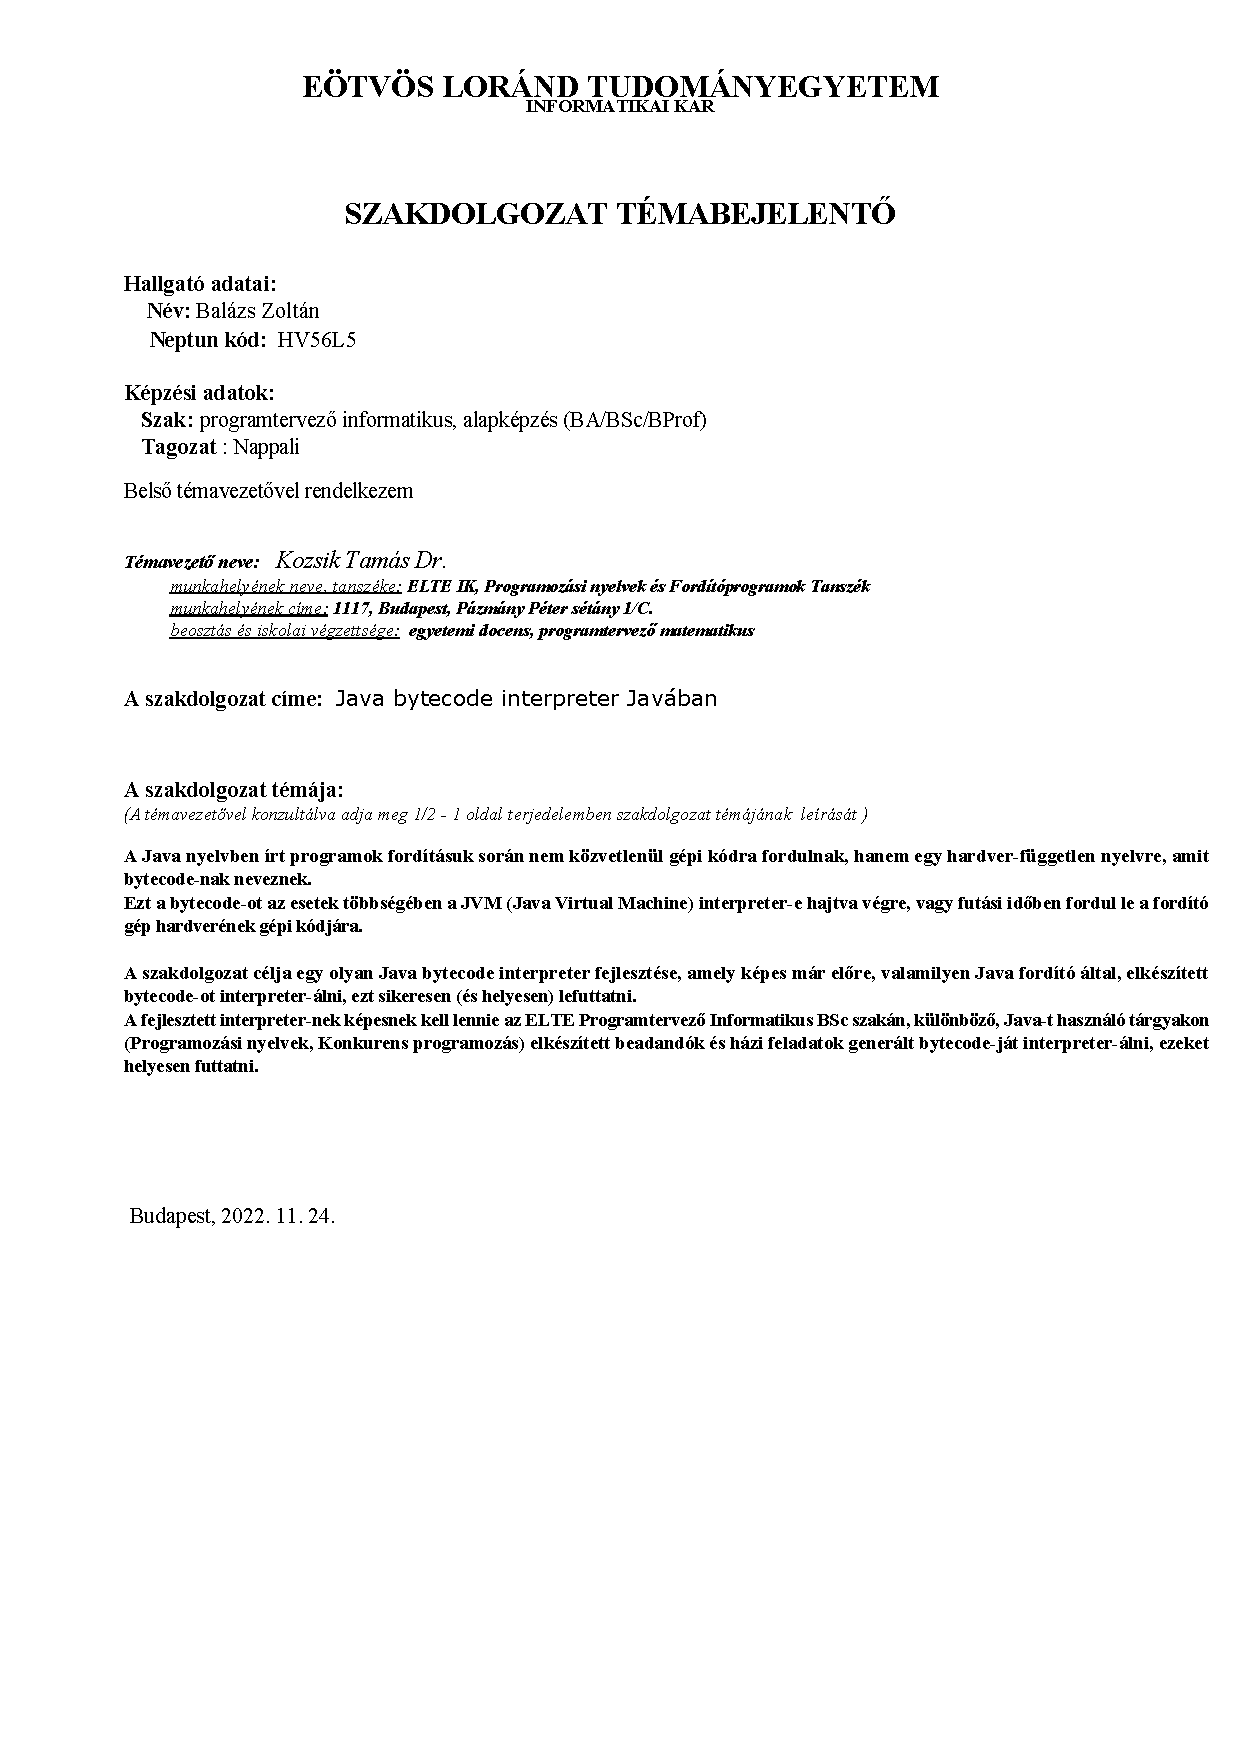
\includepdf{thesisreport.pdf}

% Table of contents (mandatory)
\tableofcontents
\cleardoublepage{}

% Main content
\chapter{Bevezetés}
\label{ch:intro}

A Java nyelvben írt programok fordításukat követően nem egy közletlen futtatható állományra (gépi kódra) fordulnak (a fordítást általában a beépített \lstinline{javac} program végzi el), hanem egy köztes nyelvre, bytecode-ra, amelyet aztán különböző programokkal az adott architektúrán interpretáljuk. Legtöbb esetben az interpretálást a JVM (Java Virtual Machine) interpretere hajtja végre (ez a beépített \lstinline{java} program).

A szakdolgozat célja egy kiegészítő program (fantázianevén \textit{Jabyinja} $-$ \textit{\textbf{Ja}va \textbf{by}tecode \textbf{in}terpreter in \textbf{Ja}va}) írása, amely ugyan hagyatkozik a \lstinline{javac} és \lstinline{java} programokra (az előbbire a fordítás, az utóbbira a futtatás miatt), de a tényleges futtatást a különböző bytecode instrukciók implementálásval végzi el.

A program nincsen Java kód interpretálásához kötve, a Java bytecode a neve ellenére más programozási nyelveknek is az alapja (ezek közül az ismertebbek: Kotlin, Clojure), viszont a tesztelés csak Java kódból generált bytecodera tér ki, ugyanis a szakdolgozat céljaként az ELTE Programtervező Informatikus BSc szakán elkészített Java programok fordításának interpretálását tűztem ki.

A programnak szükséges értelmeznie kell egy adott Classfájlt (többet is ha egy külön fájlra is hivatkozunk), helyesen beolvasnia a benne lévő adatokat, majd a belépési (\textit{main}) metódust lefuttatnia. A program erősen alapszik a Java nyelvbe beépített reflekcióra, ezen felül saját stack implementálása is szükséges. Mivel a Java nyelvre épül a program, ezért saját heap megírására nincsen szükség, ez automatikusan kezelve lesz.
\cleardoublepage{}

\chapter{Felhasználói dokumentáció}
\label{ch:user}

A program elsődleges felhasználói fejlesztők. Alapszintű tudás szükséges a Java nyelvről (vagy bármilyen olyan nyelvről amely Java bájtkódra fordul), a class fájlokról, illetve a Java programok fordításáról.

Mivel az elkészített program csak interpretálni tud, a fordítást egy már elérhető Java fordítóprogrammal szükséges megtenni. Mivel a Java programok class fájlokra fordulnak, ezek futtatásához szükséges egy interpretáló program.

Alapvető esetben ez a fordítóprogrammal együtt telepítésre kerül. A szakdolgozat esetében a lefordított class fájl futtatásával képesek lehetünk más, már lefordított Java programot futtatni.

A mellékelt fájlok között elérhető egy jar fájl is, ennek a futtatásához ugyanúgy szükségünk van egy beépített interpretáló programra (ami nem a szakdolgozat megoldása), amely képes Java programokat futtatni.

\section{Probléma megfogalmazása}

A program alapvető problémának egy class fájl értelmezését tűzi ki, a fordítás az előbb leírtakban nem a feladat része. 

A feladat megoldása egy futtatható class fájlt (vagy jar fájlt, a felhasználó szükségeinek megfelelően) eredményez, amely képes más Java class fájlokat interpretálni, azokban lévő különböző függvényeket meghívni, a \lstinline{stack}, illetve lokális változókat helyesen változtatni.

A megoldáshoz be kell olvasnia a programnak egy class fájlt, helyesen értelmezni hogy mely része mi is, majd a megfelelő részeket szekvenciálisan értelmezni, az utasításokat a specifikációnak megfelelően végrehajtani. 

\section{Megoldás rövid leírása}

A megoldás erősen alapszik a JVM specifikációra\cite{jvm_specification}, annak is a 7-es verziójára. Ebben a dokumentumban elsősorban le van írva a class fájl felépítése. Mik követik egymást, ezen belül fontos nekünk a \lstinline{Constant Pool} és a \lstinline{Methods} rész. A \lstinline{Constant Pool}-ban találunk minden olyan információt amely szükséges ahhoz, hogy milyen osztályaink, metódusaink, metódus szignatúráink és változóértékeink vannak. A \lstinline{Methods} részben találjuk a tényleges utasításokat, itt hívodnak meg a \lstinline{Constant Pool}-ban leírt osztályoknak a metódusai, itt végezzük el az értelmezést.

A programban szerepelnek a szükséges adatszerkezetek: a \lstinline{stack} és a lokális változók. Az interpretált kódot egy bájt tömbként értelmezi a program, amelyhez szükséges a jelenlegi indexet egy külön változóban eltárolnunk. Ez a változó azért is szükséges, hogy a különböző elágazások, ciklusok működni tudjanak, leegyszerűsítve a ciklus csak egy elágazás, amely többször hajtódik végre.

\section{Program használata}

\subsection{Kikötések}
A program csak Java 7-nél újabb fordítóprogrammal fordított Java programokat képes interpretálni, számos bájtkód instrukciót a Java 7-es verziójában elavulttá tettek (ezek: \lstinline{ret}, \lstinline{jsr}, \lstinline{jsr_w}), nem fordulnak elő class fájlokban. A szakdolgozat ezeket az instrukciókat nem implementálta. (Implementálásukról részletesebben szó van a fejlesztői dokumentáció "Továbbfejlesztési lehetőségek" szekciójában, implementálásuk viszonylag triviális, viszont megértésük segít elmélyülni a Java bátjkódban.)

Ezen felül egy másik, a Java 7-nél újabb verziójú programokban elég gyakran előforduló instrukció is implementálatlan maradt (név szerint az \lstinline{invokedynamic}), tehát nem minden program futtatható. Ennek az indoka hogy ez az utasítás nagyon nagy szintű elmélyülést igényel a Java bájtkódban, értelmezése meghaladja egy szakdolgozat szintjét. Ez az instrukció önmagában használható arra hogy egy, a szakdolgozat témájához hasonló, Java bátjkód interpretert írjon az ember. Ha a class fájlok egyike tartalmazza ezt az instrukciót, akkor a program jelez a felhasználó számára. Akaratlanul is része lehet a programunknak ez az instrukció, amikor egy változót szöveggel együtt próbálunk kiírni:
\begin{listing}[H]
\begin{minted}{java}
public class InvokeDynamic {
	public static void main(String[] args) {
		String world = "world";
		System.out.println("Hello " + world);
	}
}
\end{minted}
\caption{invokedynamic utasítást tartalmazó Java kód}
\end{listing}
akkor a legtöbb fordítóprogram egy \lstinline{invokedynamic} utasítást is elhelyez a programunkban.

Ez viszont elkerülhető, ha megfelelő flagekkel fordítjuk le a programunkat, mégpedig a \lstinline{-XDstringConcat=inline} flag használatával az \lstinline{invokedynamic} nem fog szerepelni a string konkatenációnál.

\subsection{Fordítástól futásig}

\subsubsection{Minimum követelmények}

A program fordításához legalább a Java 17-es verziója szükséges. Ez alatt a program fordulni sem képes, mivel pár olyan funkciót használ, amely csak a 17-es verzióban lett bevezetve.

A könnyebb fordítás (illetve egyszerűbb jar fájl készítés) érdekében a Maven fordítás automatizálási program telepítése ajánlott, ezen belül is a 3.9.0-ás verzió.

A szakdolgozatban megtalálható \lstinline{target} mappában megtalálhatóak a lefordított class fájl, illetve a jar fájl is.

\subsubsection{Fordítás}

Ha nem akarunk Maven-t használni, akkor a fordítás menete a következő:
\begin{compactitem}
	\item Menjünk a \lstinline{src/main/java} mappába (a \lstinline{$} jel arra utal, hogy normál felhasználóként futtassuk a parancsot): 
	\begin{minted}{bash}
$ cd src/main/java/
	\end{minted}
	\item Fordítsuk le a \lstinline{com/zoltanbalazs/Main.java} fájlt:
	\begin{minted}{bash}
$ javac com/zoltanbalazs/Main.java
	\end{minted}
	\item Az elkészült class fájl a \lstinline{src/main/java/com/zoltanbalazs} mappában lesz 
\end{compactitem}

Maven-t használva ez a procedúra egyszerűbb:
\begin{compactitem}
	\item Futtassuk le a csomagoló parancsot:
	\begin{minted}{bash}
$ mvn package
	\end{minted}
	\item Az elkészült class fájl a \lstinline{target/classes/com/zoltanbalazs} mappában lesz, ezen felül a \lstinline{target} mappában lesz egy futtatható jar fájl is
\end{compactitem}

\subsubsection{Futtattás}

Ha a generált class fájllal akarjuk futtatni a programot, futtassuk le a \lstinline{java com.zoltanbalazs.Main} parancsot a \lstinline{src/main/java} mappában.\ (ha Maven-nel fordítottunk akkor a \lstinline{target/classes} mappában futtassuk le a korábbi parancsot)

A Maven által készített jar fájllal való futtatáshoz, futtassuk le a \lstinline{java -jar target/jabyinja-1.0.0.jar} parancsot a főmappában.

Mindkét esetben egy opcionális argumentumot (argumentum sorozatot ha a futtatandó programunk vár parancssori argumentumot) meg tudunk adni, ez a \lstinline{main} metódust tartalmazó class fájl elérési útvonala. Alapvető esetben a program a futási mappában próbál meg egy \lstinline{Main.class} fájlt futtatni.

Futásra egy példa:
\begin{minted}{bash}
$ java -jar target/jabyinja-1.0.0.jar target/test-classes/com/zoltanbalazs/PTI/_01/Greet.class World
\end{minted}

A class fájl futtatása esetén ne felejtsük el a megfelelő class fájl elérési utat beállítani a \lstinline{cp} kapcsolóval:
\begin{minted}{bash}
$ java -cp target/classes com.zoltanbalazs.Main target/test-classes/com/zoltanbalazs/PTI/_01/Greet.class World
\end{minted}

\subsubsection{Önfuttatás}

Az elkészült interpreter képes saját magát is futtatni, ehhez a futtatáshoz hasonlóan meg kell adni a programnak a saját class fájlának elérési útját, majd opcionálisan a többi paramétert.

Ez a futtatás jar fájl esetén így néz ki, a főkönyvtárból futtatva:
\begin{minted}{bash}
$ java -jar target/jabyinja-1.0.0.jar target/classes/com/zoltanbalazs/Main.class target/test-classes/com/zoltanbalazs/PTI/_01/Greet.class World
\end{minted}

Ugyanez a class fájllal való futtatás esetén:
\begin{minted}{bash}
$ java -cp target/classes com.zoltanbalazs.Main target/classes/com/zoltanbalazs/Main.class target/test-classes/com/zoltanbalazs/PTI/_01/Greet.class World
\end{minted}

\subsection{Felmerülő problémák}

A futtatandó program futása során nem merül fel probléma (hacsak nincsen \lstinline{invokedynamic} a generált class fájlban) amelyet a program okoz. Ha a futtatandó programunk hibát dob, akkor ezt az interpretáló program is ugyanúgy megteszi; viszont a hiba kiírása során nem biztos hogy ugyanazt a kimentet kapjuk mint a beépített interpreterrel.

Tehát ha a hibánk nem egy \lstinline{try, catch} blokk-ban szerepel, akkor a kiírt üzenet nem biztos hogy ugyanaz lesz mint a beépített interpreterrel, az összes többi kiírt üzenet viszont ugyanaz kell hogy legyen.
\cleardoublepage{}

\chapter{Fejlesztői dokumentáció}
\label{ch:impl}

A program számos segítséget ad fejlesztőknek a kód egyszerű értelmezésére; a kód bővítésére. Vállalkozó szellemű embereknek a program egy teljes Java interpretert tud nyújtani viszonylag kevés továbbfejlesztéssel. A Java bájtkód instrukciók megértése során bármely Java fejlesztő jobban tudja értékelni hogy mit is csinál a Java fordítóprogram a háttérben. A program nagyon szorosan épül a JVM specifikációra, a specifikációt annak megfelelően próbálja implementálni.

\section{Class fájl felépítése}

\subsection{Class fájltól a benne levő metódus futtatásáig}

A fő osztály a \lstinline{ClassFile}, ez felel számos dologért, többek között egy class fájl beolvasáért, a megfelelő adattagok beállításával. A \lstinline{ClassFile} osztálynak egy konstruktora van, mégpedig:
\begin{minted}{java}
public ClassFile(String fileName, String[] mainArgs)
\end{minted}
Tehát az első paraméter a beolvasandó class fájl neve, a második pedig a \lstinline{main} metódusnak adott argumentumok.

Az implementáció alapján nem kötött a \lstinline{main} metódus használata belépési pontként, tehát a 2.\ argumentum lehet \lstinline{null} is.

A konstruktor meghívása egyidejüleg meghívja a \lstinline{readClassFile} függvényt is:
\begin{minted}{java}
public void readClassFile(String fileName)
\end{minted}
Ez a függvény egy adott fájlnévre beolvassa a class fájlban tárolt adatokat megfelelő változókba.
(Ezen felül egy \lstinline{VALID_CLASS_FILE} változót is beállít; feltétellezük hogy ha a mágikus szám \lstinline{(CA FE BA BE)} megtalálható a fájl elején, akkor az adott fájl egy valid class fájl, ellenkező esetben egy \lstinline{InvalidClassFileException}-t dob a beolvasó függvény.)

A beolvasás után (tehát az objektum létrehozása után) érdemes a belépési függvényt (általában \lstinline{main}) megkeresni a \lstinline{findMethodsByName} metódussal:
\begin{minted}{java}
public Method_Info findMethodsByName(String methodName)
\end{minted}
Ez egy adott függvénynévre a megfelelő nevü metódust visszaadja a beolvasott fájlból (ha nem talál ilyet akkor \lstinline{null}-t ad vissza).
Egy példa a használatára:
\begin{minted}{java}
ClassFile CLASS_FILE = new ClassFile("Main.class", null);
Method_Info method = CLASS_FILE.findMethodsByName("main");
\end{minted}

A függvény megtalálása után ajánlott a \lstinline{Code} attribútumot megtalálni, ebben, többek között, található a futtatandó Java bájtkód is. A segédfüggvény erre a \lstinline{findAttributesByName}:
\begin{minted}{java}
public List<Attribute_Info> findAttributesByName(List<Attribute_Info> attributes, String attributeName)
\end{minted}
Mivel egy attribútumból több is lehet, egy listát kapunk vissza (a \lstinline{Code}-ból csak egy lesz), bemeneti paraméterként az attribútumnév mellett a megfelelü függvény attribútumait is át kell adnuk, például:
\begin{minted}{java}
List<Attribute_Info> attributes = CLASS_FILE.findAttributesByName(method.attributes, "Code");
\end{minted}
(Ha nem talál ilyen nevezetű attribútumot akkor üres listát ad vissza.)

A megfelelüen beolvasott attribútum után, a megtalált attribútumok között ajanlott végigmenni, a \lstinline{List} implementálja az \lstinline{Iterable}-t, így egy for ciklussal elegánsan megtehetjük ezt:
\begin{minted}{java}
for (Attribute_Info attribute : attributes)
\end{minted}

Mivel \lstinline{Code} attribútumokról beszélünk, ezért a következő ajánlott dolog hogy ebből az attribútumból olvassuk be az adatokat. Ehhez a \lstinline{Code_Attribute_Helper} osztály \lstinline{readCodeAttributes} metódusa megfelelő:
\begin{minted}{java}
public static Code_Attribute readCodeAttributes(Attribute_Info attribute) throws IOException
\end{minted}
A függvény egy attribútumot vár (például az előbbi kódrészlet \lstinline{attribute} változóját), majd pedig beolvassa a specifikációnak megfelelően a \lstinline{Code_Attribute}-ot, és visszaadja azt, ha valamiért nem sikerült a beolvasás akkor \lstinline{IOException}-t dob a függvény.
\begin{minted}{java}
Code_Attribute codeAttribute = Code_Attribute_Helper.readCodeAttributes(attribute);
\end{minted}

Ezt a beolvasott attribútumot a \lstinline{ClassFile} osztály fel tudja használni az \lstinline{executeCode} metódusával, mely egy \lstinline{byte[]} változót vár bemeneti paraméterként, ami a \lstinline{Code_Attribute} része:
\begin{minted}{java}
public Pair<Class<?>, Object> executeCode(byte[] code)
	throws IOException, ClassNotFoundException, NoSuchFieldException, IllegalAccessException,
	NoSuchMethodException, SecurityException, InstantiationException, IllegalArgumentException,
	InvocationTargetException, Throwable
\end{minted}
A reflekció miatt számos hibát dob vissza a függvény, ha nem helyes a kód formátuma akkor \lstinline{IOException}-t dob a függvény, a \lstinline{Throwable} az \lstinline{ATHROW} Java bájtkód instrukció miatt szükséges (ekkor egy hibát dob vissza a metódusunk).
Visszatérési értéke \lstinline{Pair<Class<?>, Object>}, a számos \lstinline{RETURN} utasítás miatt (ezeket a stack-en szükséges elhelyezünk)
Példa a használatára:
\begin{minted}{java}
CLASS_FILE.executeCode(codeAttribute.code);
\end{minted}

Ezzel el is jutottunk egy class fájl beolvasásától, az abban lévő adott függvény Java bájtkódjának futtatásáig, több teendőnk nincsen, a program az adott függvényben levő külön függvényhívásokat automatikusan elvégzi.

A teljes példakód:
\begin{minted}{java}
ClassFile CLASS_FILE = new ClassFile("Main.class", null);
Method_Info method = CLASS_FILE.findMethodsByName("main");
List<Attribute_Info> attributes = CLASS_FILE.findAttributesByName(method.attributes, "Code");

for (Attribute_Info attribute : attributes) {
	Code_Attribute codeAttribute = Code_Attribute_Helper.readCodeAttributes(attribute);
	CLASS_FILE.executeCode(codeAttribute.code);
}
\end{minted}

\subsection{Pár minta class fájl felépítése}

A legegyszerűbb class fájl ami értelmes, viszont nem futattható:

\begin{center}
\begin{tabular}{ c c c c c c c c c c c c c c c }
\stagemagic{CA} & \stagemagic{FE} & \stagemagic{BA} & \stagemagic{BE} & \stageminor{00} & \stageminor{00} & \stagemajor{00} & \stagemajor{00} & \stageconstantsize{00} & \stageconstantsize{00} & \stageaccessflags{00} & \stageaccessflags{00} & \stagethisclass{00} & \stagethisclass{00} & \stagesuperclass{00} \\
\stagesuperclass{00} & \stageinterfacesize{00} & \stageinterfacesize{00} & \stagefieldsize{00} & \stagefieldsize{00} & \stagemethodsize{00} & \stagemethodsize{00} & \stageattributes{00} & \stageattributes{00}
\end{tabular}
\end{center}

Java kódban ennek megfelelője az üres fájl:
\begin{minted}{java}
\end{minted}

Class fájl formátumának magyarázata:

\begin{compactitem}
\setlength\itemsep{-5px}
\item \stagemagic{CA FE BA BE}: Mágikus szám, amely minden Class fájl elején megtalálható
\item \stageminor{00 00} \stagemajor{00 00}: Class fájl \lstinline{Minor} és \lstinline{Major} verziószáma, egy táblázatnak megfelelően a fordítóprogram verziója
\item \stageconstantsize{00 00}: A Constant Pool mérete (+1, mivel 1-től indexelt, itt nem számít)
\item \stageaccessflags{00 00}: Hozzáférési zászlók ()
\item \stagethisclass{00 00}: \lstinline{This} osztály indexe a Constant Pool-ban
\item \stagesuperclass{00 00}: \lstinline{Super} osztály indexe a Constant Pool-ban
\item \stageinterfacesize{00 00}: Interfészek száma
\item \stagefieldsize{00 00}: Adattagok száma
\item \stagemethodsize{00 00}: Függvények száma
\item \stageattributes{00 00}: Osztály attribútumainak száma
\end{compactitem}

\pagebreak

A legegyszerűbb class fájl amit a $Jabyinja$ program le tud futtatni (a beépített \lstinline{java} program nem képes ezt lefuttatni, mivel nincsenek benne osztályok, a JVM specifikáció alapján az osztályok elhanyagolhatóak):

\begin{center}
\begin{tabular}{ c c c c c c c c c c c c c c c }
\stagemagic{CA} & \stagemagic{FE} & \stagemagic{BA} & \stagemagic{BE} & \stageminor{00} & \stageminor{00} & \stagemajor{00} & \stagemajor{00} & \stageconstantsize{00} & \stageconstantsize{04} & \stageconstantpool{01} & \stageconstantpool{00} & \stageconstantpool{04} & \stageconstantpool{43} & \stageconstantpool{6F} \\
\stageconstantpool{64} & \stageconstantpool{65} & \stageconstantpool{01} & \stageconstantpool{00} & \stageconstantpool{04} & \stageconstantpool{6D} & \stageconstantpool{61} & \stageconstantpool{69} & \stageconstantpool{6E} & \stageconstantpool{01} & \stageconstantpool{00} & \stageconstantpool{03} & \stageconstantpool{28} & \stageconstantpool{29} & \stageconstantpool{56} \\
\stageaccessflags{00} & \stageaccessflags{21} & \stagethisclass{00} & \stagethisclass{00} & \stagesuperclass{00} & \stagesuperclass{00} & \stageinterfacesize{00} & \stageinterfacesize{00} & \stagefieldsize{00} & \stagefieldsize{00} & \stagemethodsize{00} & \stagemethodsize{01} & \stagemethods{00} & \stagemethods{09} & \stagemethods{00} \\ 
\stagemethods{02} & \stagemethods{00} & \stagemethods{03} & \stagemethods{00} & \stagemethods{01} & \stagemethods{00} & \stagemethods{01} & \stagemethods{00} & \stagemethods{00} & \stagemethods{00} & \stagemethods{0D} & \stagemethods{00} & \stagemethods{00} & \stagemethods{00} & \stagemethods{00} \\
\stagemethods{00} & \stagemethods{00} & \stagemethods{00} & \stagemethods{01} & \stagemethods{B1} & \stagemethods{00} & \stagemethods{00} & \stagemethods{00} & \stagemethods{00} & \stageattributes{00} & \stageattributes{00}
\end{tabular}
\end{center}

Java kód megfelelője:
\begin{minted}{java}
public static void main() {
    return;
}
\end{minted}

Class fájl formátumának magyarázata:

\begin{compactitem}
\setlength\itemsep{-5px}
\item \stagemagic{CA FE BA BE}: Mágikus szám, amely minden class fájl elején megtalálható
\item \stageminor{00 00} \stagemajor{00 00}: Class fájl \lstinline{Minor} és \lstinline{Major} verziószáma, egy táblázatnak megfelelően a \lstinline{javac} fordítóprogram verziója
\item \stageconstantsize{00 04}: A Constant Pool mérete (+1, mivel 1-től indexelt)
\item \stageconstantpool{01 00 04 43 6F 64 65 01 00 04 6D 61 69 6E 01 00 03 28 29 56}: Constant Pool
\begin{compactitem}
    \setlength\itemsep{-5px}
    \item \stagemajor{01} \stageminor{00 04} \stageconstantsize{43 6F 64 65} \\
    \stagemajor{01}: Constant Pool Info érték \lstinline{(CONSTANT_Utf8)} \\
    \stageminor{00 04}: 4 hosszú \\
    \stageconstantsize{43 6F 64 65}: A \lstinline{CONSTANT_Utf8} értéke: \lstinline{Code}
    \item \stagemajor{01} \stageminor{00 04} \stageconstantsize{6D 61 69 6E} \\
    \stagemajor{01}: Constant Pool Info érték \lstinline{(CONSTANT_Utf8)} \\
    \stageminor{00 04}: 4 hosszú \\
    \stageconstantsize{6D 61 69 6E}: A \lstinline{CONSTANT_Utf8} értéke: \lstinline{main}
    \item \stagemajor{01} \stageminor{00 03} \stageconstantsize{28 29 56} \\
    \stagemajor{01}: Constant Pool Info érték \lstinline{(CONSTANT_Utf8)} \\
    \stageminor{00 03}: 3 hosszú \\
    \stageconstantsize{28 29 56}: A \lstinline{CONSTANT_Utf8} értéke: \lstinline{()V}
\end{compactitem}
\item \stageaccessflags{00 21}: Hozzáférési zászlók \lstinline{(Public, Super)} - elhanyagolhatóak ebben az esetben
\item \stagethisclass{00 00}: \lstinline{This} osztály indexe a Constant Pool-ban
\item \stagesuperclass{00 00}: \lstinline{Super} osztály indexe a Constant Pool-ban
\item \stageinterfacesize{00 00}: Interfészek száma
\item \stagefieldsize{00 00}: Adattagok száma
\item \stagemethodsize{00 01}: Függvények száma
\item \stagemethods{00 09 00 02 00 03 00 01 00 01 00 00 00 0D 00 00 00 00 00 00 00 01 B1 00 00 00 00}: Függvények
\begin{compactitem}
    \setlength\itemsep{-5px}
    \item \stagemajor{00 09} \stageminor{00 02} \stageconstantsize{00 03} \stageconstantpool{00 01} \stageaccessflags{00 01 00 00 00 0D 00 00 00 00 00 00 00 01 B1 00 00 00 00} \\
    \stagemajor{00 09}: Hozzáférési zászlók \lstinline{(Public, Static)} \\
    \stageminor{00 02}: Constant Poolban lévő indexe a függvénynek: \lstinline{main} \\
    \stageconstantsize{00 03}: Függvény leírása (bemeneti paraméterek, visszatérési érték): \lstinline{()V} \\
    \stageconstantpool{00 01}: Függvény attribútumainak száma \\
    \stageaccessflags{00 01 00 00 00 0D 00 00 00 00 00 00 00 01 B1 00 00 00 00}: Attribútumok
    \begin{compactitem}
        \setlength\itemsep{-5px}
        \item[•] \stagemajor{00 01} \stageminor{00 00 00 0D} \stageconstantsize{00 00 00 00 00 00 00 01 B1 00 00 00 00} \\
        \stagemajor{00 01}: Constant Pool-ban lévő indexe az attribútumnak: \lstinline{Code} \\
        \stageminor{00 00 00 0D}: Attribútum hossza (\lstinline{0D} = 13 bájt) \\
        \stageconstantsize{00 00 00 00 00 00 00 01 B1 00 00 00 00}: Attribútum
            \begin{compactitem}
            \setlength\itemsep{0px}
                \item[–] \stagemajor{00 00} \stageminor{00 00} \stageconstantsize{00 00 00 01} \stageconstantpool{B1} \stageaccessflags{00 00} \stagethisclass{00 00} \\
                \stagemajor{00 00}: Stack mérete  \\
                \stageminor{00 00}: Lokális változók száma \\
                \stageconstantsize{00 00 00 01}: Kód hossza \\
                \stageconstantpool{B1}: Kód \lstinline{(B1 = return)}  \\
                \stageaccessflags{00 00}: Kivételek száma \\
                \stagethisclass{00 00}: Attribútum attribútumainak száma
        \end{compactitem}
    \end{compactitem}
\end{compactitem}
\item \stageattributes{00 00}: Osztály attribútumainak száma
\end{compactitem}

\subsection{Adatszerkezetek}

A class fájlnak megfelelően a két legfontosabb adattag a \lstinline{stack} és a \lstinline{local} (lokális) változók. A különböző instrukciók az ezeken lévő adatokkal dolgoznak, erre/ebbe helyeznek el megfelelő adatokat.

Az egyszerűség kedvéért a \lstinline{stack} reprezentációjában az osztály típusát is elmentjük, a két adattag Java reprezentációja a \lstinline{ClassFile} osztályban:
\begin{minted}{java}
public List<Pair<Class<?>, Object>> stack = new ArrayList<>();
public Object[] local = new Object[65536];
\end{minted}
(A \lstinline{Pair} egy egyedi osztály, mely két adattagot tud eltárolni, más nyelvekben \lstinline{tuple}-ként is ismeretes.)

A lokális változók maximális mennyiségét előre tudjuk, ez nem lehet több mint egy 16-bites előjel nélküli szám ($2^{16} = 65536$), alapból ennek az értéke egy 8-bites előjel nélküli szám ($2^8 = 256$) lenne, mivel a \lstinline{store} és \lstinline{load} utasításokat csak egy 8-bites előjel nélküli szám (az \lstinline{index}) követi, viszont a \lstinline{wide} utasítással a \lstinline{store} és \lstinline{load} utasítások módosíthatóak, hogy 2 db 8-bites előjel nélküli számot olvassanak be, tehát lényegében egy 16-bites előjel nélküli számot.

Gyakorlatban ez a szám csökkenthető lenne, tudhatjuk hogy futási időben mennyi lokális változója (illetve a \lstinline{stack} nagyságát is tudhatjuk, tehát tömbként is reprezentálhatnánk) van egy metódusnak. Ez bővebben le van írva a továbbfejlesztési lehetőségekben.

Kényelmi szempontból létezik a \lstinline{CodeIndex} osztály, amely lényegében egy \lstinline{int} szám absztrakciója:
\begin{minted}{java}
class CodeIndex {
    private int index = 0;

    public void Inc(int value) {
        index += value;
    }

    public int Next() {
        return index++;
    }

    public void Set(int value) {
        index = value;
    }

    public int Get() {
        return index;
    }
}
\end{minted}
Az absztrakció oka hogy függvényeknek átadva lehessen módosítani ezt a számot; a szám a jelenlegi index a kódot reprezentáló \lstinline{byte} tömbben, megmondja hogy a tömbben lévő melyik indexen levő instrukciót kell végrehajtani.

Az absztrakció különösen észrevehető amikor az \lstinline{if} és \lstinline{goto} utasításokat hajtjuk végre, a \lstinline{ClassFile} objektumunk lokális változója módosítható az \lstinline{Instructions} osztály metódusain keresztül. Mivel a Java érték szerint adja át a paramétereket, ez egy sima \lstinline{int} számmal nem lehetne megoldani.

\subsection{Interpretálás algoritmusa}

Az \ref{alg:ibb}.~algoritmus egy általános elágazás és korlátozás algoritmust (\emph{Branch and Bound algorithm}) mutat be. A \ref{step:selrule}.~lépésben egy megfelelő kiválasztási szabályt kell alkalmazni.
Példa forrása: \href{https://www.inf.u-szeged.hu/actacybernetica/}{Acta Cybernetica (ez egy hiperlink)}.

\begin{algorithm}[H]
\caption{A general interval B\&B algorithm}
\label{alg:ibb}
\textbf{\underline{Funct}} IBB($S,f$)
\begin{algorithmic}[1] % sorszámok megjelenítése minden n. sor előtt, most n = 1
\State Set the working list ${\cal L}_W$ := $\{S\}$ and the final list ${\cal L}_Q$ := $\{\}$
\While{( ${\cal L}_W \neq \emptyset$ )} \label{alg:igoend}
	\State Select an interval $X$ from ${\cal L}_W$ \label{step:selrule}\Comment{Selection rule}
	\State Compute $lbf(X)$ \Comment{Bounding rule}
	\If{$X$ cannot be eliminated} \Comment{Elimination rule}
		\State Divide $X$ into $X^j,\ j=1,\dots, p$, subintervals   \Comment{Division rule}
		\For{$j=1,\ldots,p$}
			\If{$X^j$ satisfies the termination criterion} \Comment{Termination rule}
				\State Store $X^j$ in ${\cal L}_W$
			\Else
				\State Store $X^j$ in ${\cal L}_W$
			\EndIf
		\EndFor
	\EndIf
\EndWhile
\State \textbf{return} ${\cal L}_Q$
\end{algorithmic}
\end{algorithm}

\section{Az interpreter sajátosságai}

\subsection{Erőforrás igények}

A \lstinline{Linux} operációs rendszeren beépített \lstinline{time} programot (illetve a \lstinline{hyperfine} programot) használva az erőforrás igények a tesztfájlokra az alábbiak (a tesztelt számítógép releváns specifikációi: Intel Core i7-8700k processzor 4.7 GHz-en, 16 GB DDR4 memória 2133 MT/s sebességgel):

\begin{center}
	\centering
	\begin{longtable}{ | l | r | r | r | r | }

		\hline
		\multirow{2}{*}{\textbf{Tesztfájl}} & \multicolumn{2}{ c | }{\textbf{/usr/bin/java}} & \multicolumn{2}{ c | }{\textbf{Jabyinja}} \\
		\cline{2-5}
		& Memória & Futási idő & Memória & Futási idő \\
		\hline \hline		
		\endfirsthead

		\hline
		\multirow{2}{*}{\textbf{Tesztfájl}} & \multicolumn{2}{ c | }{\textbf{/usr/bin/java}} & \multicolumn{2}{ c | }{\textbf{Jabyinja}} \\
		\cline{2-5}
		& Memória & Futási idő & Memória & Futási idő \\
		\hline \hline		
		\endhead

		Own/Arithmetic.class & 37,1 MB & 21,4 ms & 47,6 MB & 92,8 ms \\
		\hline
		Own/Arrayclass.class & 34,9 MB & 20,9 ms & 54,6 MB & 130,8 ms \\
		\hline
		Own/Arraylist.class & 37,2 MB & 21,4 ms & 49,6 MB & 87,1 ms \\
		\hline
		Own/Athrow.class & 34,6 MB & 20,4 ms & 46,9 MB & 61,7 ms \\
		\hline
		Own/Dup2.class & 36,3 MB & 20,3 ms & 39,2 MB & 45,6 ms \\
		\hline
		Own/Inheritence.class & 34,8 MB & 20,7 ms & 51,9 MB & 98,1 ms \\
		\hline
		Own/Instanceof.class & 38,8 MB & 20,2 ms & 43,1 MB & 64,2 ms \\
		\hline
		Own/Multianewarray.class & 34,4 MB & 20,6 ms & 47,7 MB & 62,9 ms \\
		\hline
		Own/Nested.class & 39,3 MB & 22,1 ms & 47,2 MB & 80,5 ms \\
		\hline
		Own/Ownclass.class & 37,5 MB & 20,2 ms & 61,9 MB & 135,5 ms \\
		\hline
		Own/SwitchAthrow.class & 36,8 MB & 20,5 ms & 40,5 MB & 43,9 ms \\
		\hline
		Own/Template.class & 39,2 MB & 21,2 ms & 51,9 MB & 86,5 ms \\
		\hline
		PTI/\_01/Euler.class & 39,5 MB & 22,1 ms & 47,5 MB & 66,4 ms \\
		\hline
		PTI/\_01/Factorial.class & 39,6 MB & 21,8 ms & 50,7 MB & 68,4 ms \\
		\hline
		PTI/\_01/GCD.class & 38,9 MB & 20,6 ms & 51,6 MB & 67,8 ms \\
		\hline
		PTI/\_01/Greet.class & 38,8 MB & 20,8 ms & 50,8 MB & 56,8 ms \\
		\hline
		PTI/\_01/Half.class & 39,6 MB & 22,7 ms & 50,7 MB & 69,7 ms \\
		\hline
		PTI/\_01/Odd.class & 38,5 MB & 20,7 ms & 37,8 MB & 69,7 ms \\
		\hline
		PTI/\_01/PerfectNum.class & 38,8 MB & 20,7 ms & 51,2 MB & 57,1 ms \\
		\hline
		PTI/\_01/PerfectNumRange.class & 37,8 MB & 20,6 ms & 70,6 MB & 87,6 ms \\
		\hline
		PTI/\_01/Print.class & 41,1 MB & 21,4 ms & 51,2 MB & 67,2 ms \\
		\hline
		PTI/\_01/Sqrt.class & 35,7 MB & 22,3 ms & 50,9 MB & 70,3 ms \\
		\hline
		PTI/\_01/SquareRoot.class & 37,6 MB & 22,4 ms & 43,1 MB & 71,5 ms \\
		\hline
		PTI/\_01/TwoNum.class & 35,1 MB & 20,6 ms & 47,7 MB & 75,8 ms \\
		\hline
		PTI/\_02/\_01/PointMain.class & 41,5 MB & 22,3 ms & 55,6 MB & 122,7 ms \\
		\hline
		PTI/\_02/\_02/CircleMain.class & 41,5 MB & 21,3 ms & 53,1 MB & 82,5 ms \\
		\hline
		PTI/\_02/\_03/CircleMain.class & 41,3 MB & 22,7 ms & 55,1 MB & 93,7 ms \\
		\hline
		PTI/\_02/\_04/ComplexMain.class & 41,5 MB & 21,2 ms & 58,4 MB & 125,7 ms \\
		\hline
		PTI/\_02/\_05/LineMain.class & 41,4 MB & 20,7 ms & 56,7 MB & 102,5 ms \\
		\hline
		PTI/\_03/IterletterMain.class & 41,7 MB & 20,8 ms & 78,9 MB & 180,5 ms \\
		\hline
		PTI/\_04/\_01/PointMain.class & 39,6 MB & 22,7 ms & 58,8 MB & 126,7 ms \\
		\hline
		PTI/\_04/\_02/DoubleVectorMain.class & 41,3 MB & 21,1 ms & 68,5 MB & 176,2 ms \\
		\hline
		PTI/\_05/\_01/Swap.class & 41,2 MB & 20,1 ms & 51,9 MB & 60,5 ms \\
		\hline
		PTI/\_05/\_02/IntegerMatrixMain.class & 41,2 MB & 20,7 ms & 46,8 MB & 70,1 ms \\
		\hline
		PTI/\_05/\_03/WildAnimalMain.class & 41,0 MB & 21,2 ms & 73,4 MB & 183,5 ms \\
		\hline
		PTI/\_05/\_04/IntVectorMain.class & 43,2 MB & 21,0 ms & 53,9 MB & 93,9 ms \\
		\hline
		PTI/\_06/\_01/Calculator.class & 39,1 MB & 21,1 ms & 51,6 MB & 64,1 ms \\
		\hline
		PTI/\_06/\_02/AddByLine.class & 41,2 MB & 21,6 ms & 53,0 MB & 92,3 ms \\
		\hline
		PTI/\_06/\_03/IsPartOf.class & 39,3 MB & 22,4 ms & 51,8 MB & 73,9 ms \\
		\hline
		PTI/\_06/\_04/CircleMain.class & 41,3 MB & 22,0 ms & 64,7 MB & 124,8 ms \\
		\hline
		PTI/\_08/\_01/BookMain.class & 41,4 MB & 21,4 ms & 74,3 MB & 197,6 ms \\
		\hline
		PTI/\_08/\_02/CoffeeShop.class & 41,1 MB & 21,2 ms & 60,8 MB & 123,7 ms \\
		\hline
		PTI/\_09/\_01/Divisors.class & 41,2 MB & 20,2 ms & 52,2 MB & 85,4 ms \\
		\hline
		PTI/\_09/\_04/MultiSetMain.class & 41,4 MB & 21,6 ms & 67,7 MB & 175,4 ms \\
		\hline
		PTI/\_10/\_01/Extends.class & 41,4 MB & 20,6 ms & 52,6 MB & 82,4 ms \\
		\hline
		PTI/\_10/\_02/BookMain.class & 41,1 MB & 22,3 ms & 85,0 MB & 254,5 ms \\
		\hline
		PTI/\_10/\_03/BagMain.class & 41,4 MB & 21,4 ms & 72,7 MB & 175,2 ms \\
		\hline
		PTI/\_10/\_04/Swap.class & 41,6 MB & 20,3 ms & 53,6 MB & 101,0 ms \\
		\hline
		PTI/\_11/\_01/FlyingMain.class & 41,4 MB & 21,5 ms & 54,3 MB & 92,0 ms \\
		\hline
		PTI/\_11/\_02/Main.class & 41,3 MB & 20,8 ms & 71,6 MB & 153,7 ms \\
		\hline
		PTI/\_11/\_03/AnimalMain.class & 41,6 MB & 20,5 ms & 52,1 MB & 78,3 ms \\
		\hline
		PTI/\_11/\_04/AnimalMain.class & 41,3 MB & 21,7 ms & 64,5 MB & 152,3 ms \\
		\hline
		PTI/\_12/Inheritence.class & 41,6 MB & 20,2 ms & 47,7 MB & 68,3 ms \\
		\hline

		\caption[Erőforrás különbségek]{A beépített \lstinline{java} és az interpreter közötti erőforrás különbségek}
		\label{jabyinja:resource}
	\end{longtable}
\end{center}

\subsection{A program memóriamodellje}

A heap memória nincsen implementálva a programban. Ez alapszik a standard Java interperet implementációjára. Ide tartoznak többek között az objektumoknak a referenciái. Ebből következően a szemétgyűjtés (\lstinline{garbage collector}) a beépített Java szemétgyűjtő algoritmust alkalmazza.

A stack memória fontos építőeleme a programnak, az implementációja \lstinline{ArrayList} osztállyal van megoldva.
\begin{minted}{java}
public List<Pair<Class<?>, Object>> stack = new ArrayList<>();
\end{minted}
Ez az \lstinline{ArrayList} egy \lstinline{Class<?>}-t és \lstinline{Object}-et tartalmazó \lstinline{Pair}-eket (\lstinline{tuple}) foglal magába. Az \lstinline{Object} a konkrét érték amit a stack-en tárolni szeretnénk, a \lstinline{Class<?>} egy kényelmi megoldás miatt a tárolt értéknek a típusa.

Az implementációból következően lényegében a tényleges program-ban az alábbi memóriaeloszlás következik be:

\subsection{Az önfuttatásról}

Habár a program tényleg képes önmagát lefuttatni, a Java programozási nyelvet mélyebben értő emberek észrevehetik, hogy ez egy erősen kikötéses állítás. Mivel a beépített osztályokat nem interpretálja a program, ezért amikor egy olyan parancsot hívunk meg, mint például: 
\begin{minted}{bash}
$ java -jar target/jabyinja-1.0.0.jar target/classes/com/zoltanbalazs/Main.class target/test-classes/com/zoltanbalazs/PTI/_01/Greet.class World
\end{minted}
akkor igazából csak az interperet \lstinline{main} metódusáig interpretáljuk azt.

A \lstinline{java} beépített interperet működése miatt amikor egy jar fájlt futtatunk, minden, a jar fájlban lévő, osztály beépített lesz. Az eddig leírtak alapján pedig a beépített osztályok metódusai pedig reflekcióval vannak meghívva.

Természetesen a \lstinline{main} függvényben is megfelelően kell felépíteni a különböző adattagokat, tehát az interpret tényleg saját magát futtatja, viszont nem látunk akkora erőforrásbeli különbséget mint ami a beépített interpretert és a megírt program között van.

\section{Továbbfejlesztési lehetőségek}

\subsection{Invokedynamic utasítás}

Az egyik legszembetűnőbb hiány a szakdolgozatban az egyik nem implementált utasítás, az \lstinline{invokedynamic}, hiánya.
Ez az utasítás számos helyen előfordul Java programokban, leginkább a lambda kifejezésekben (ezen belül is a Konkurens programozás tárgyon megismert \lstinline{Executor} osztály paramétereként), illetve a kiírás során szöveg(ek) és változó(k) konkatenációjánál is ez használt.

Az utóbbi egyszerűen kiküszöbölhető a \lstinline{-XDstringConcat=inline} flag-gel való fordítás során az \lstinline{invokedynamic} utasítás lecserélődik \lstinline{StringBuilder}-en keresztül lévő \lstinline{invokevirtual} és \lstinline{invokespecial} hívásokra.

Az előző viszont sajnos jelen állapotban nem megoldott, és nem is oldható meg egyszerűen. Ahhoz hogy lambda függvények működjenek, az \lstinline{invokedynamic}-ot implementálni kell. Ehhez már az alapvető előkészület megvan, a class fájlban lévő \lstinline{bootstrap} metódusok egy külön adattag elemeiként el vannak helyezve. A továbbfejlesztés során csak a megfelelő \lstinline{CallSite} helyet, illetve a class fájlban lévő constant pool általi \lstinline{index}-eken levő metódusokkal (illetve paraméterekkel) kell meghívni az éppen leírt függvényt.

\subsection{Java 7 előtti verziók támogatása}

Viszonylag egyszerűen továbbfejleszthető a program hogy Java 7 előtti verzióval fordított class fájlokat is támogasson.

A hiányzó utasítások a \lstinline{ret}, \lstinline{jsr}, \lstinline{jsr_w}, ezek mindegyikéhez csak az szükséges, hogy a megfelelő index-re ugorjunk, a \lstinline{jsr} és \lstinline{jsr_w} utasítások során a visszatérési címet pedig a \lstinline{stack}-re helyezzük.

Természetesen mindegyik utasítás során a megfelelő index-et is be kell olvasnunk a class fájlból, amely a lokális változó megfelelő indexére (\lstinline{ret}), vagy egy adott számot (\lstinline{jsr}, \lstinline{jsr_w}) határoz meg, amely a visszatérési cím, illetve az ugrási cím.

\subsection{Optimalizálás}

A futási idő táblázata alapján látható hogy a program exponenciálisan lassabb, mint a beépített \lstinline{java} interpretáló program. A program több memóriát is igényel mint szükséges lenne. Ezeknek számos oka is van, ezek közül pár:

\begin{compactitem}
	\item A nem beépített osztályok megfelelő konstruktorait minden egyes alkalommal a program egyesével keresi ki a program. Ez a limitáció nagyon szembetűnő ha sok saját osztállyal dolgozunk. Ilyenkor a futási idő exponenciálisan lassul. Egy lehetséges megoldás erre hogy a megfelelő konstruktorokat elmenti a program, majd keresés előtt az elmentett konstruktorok között megnézzük hogy szerepel-e már a jelenleg hívandó konstruktor. Ha igen, akkor egyértelmű módon nem keressük ki, hanem felhasználjuk azt, ha nem, akkor pedig megkeressük.
	\item A \lstinline{local} változóknak maximális értéket ($65536$) foglal a program minden nem beépített függvény meghívása során, viszont a class fájlban ennek a maximális értéke le van írva a megfelelő függvény attribútumaként. Tehát a megoldás erre viszonylag egyszerű, függvényfuttatás előtt kellene a lokális változók mennyiségét beállítani. Ennek a problémának a másik verziója, hogy habár a stack egy \lstinline{LIFO} (\textit{\textbf{L}ast \textbf{I}n \textbf{F}irst \textbf{O}ut}, amely adat utoljára kerül bele, az kerül elsőnek ki belőle) adatszerkezet, a maximális mérete ennek is a class fájlban a függvény egy megfelelő attribútumaként jelen van. A már megírt függvényekkel viszonylag triviális ezt lekérdezni. (A megfelelő függvény a \lstinline{ClassFile} osztályban található \lstinline{findAttributesByName})
	\item A különböző class fájlok beolvasásának eredménye nincs elmentve, ha egy fájlt be kell olvasnunk, akkor azt minden egyes alkalommal külön-külön megteszünk, ha az eredményt elmentenénk akkor drasztikusan lehetne a sebességen gyorsítani. Ennek megoldásaként a \lstinline{Main} osztályban egy listában fel lehetne venni a beolvasott class fájlokat, egy nem beépített class fájlban levő metódus interpretálása előtt pedig végig lehetne menni a már beolvasott fájlokon. Ezzel jóval kevesebb fájl beolvasás műveletet végeznénk, cserébe a listán való végigmenés lehet hogy kevés class fájl használata esetén negatív hatással lenne.
	\item A reflekciót újragondolva, azt elhagyva a sebesség növelhető lenne, erről részletesebben a "Reflekció újragondolása" szekcióban van írva. Lényege, hogy a jelenlegi, beépített osztályokon levő reflekciót le kellene cserélni interpretálása. Az alapok ehhez megvannak, viszont ez is egy komolyabb programozási feladat.
\end{compactitem}

\subsection{További tesztelés}

A szakdolgozat írása során megpróbáltam az alapos tesztelésre figyelni, ezért is vannak az alapvető instrukciót egyesével tesztelve (minden tesztfájl-ban külön-külön instrukciók szerepelnek). Viszont a tökéletes program nem létezik, elképzelhető hogy valahol nincs megfelelően a \lstinline{stack} törölve, vagy valamely instrukció mégsem helyes. Tehát a programban elképzelhető a probléma. Ezt a még alaposabb teszteléssel minél inkább meg lehetne cáfolni.

Ehhez egy példa még több tesztfájl mellékelése. A tesztelő környezetbe (Python szkript) viszonylag egyszerűen be lehet helyezni új teszt fájlokat, amely leellenőrzi hogy megfelelő-e a program futása. Továbbfejlesztésként lehet Java programokat írni, majd ezeket a tesztelő környezethez hozzáadni, és ellenőrizni hogy jól fut-e le a program.

Egy másik érdekes továbbfejlesztés, hogy ne csak Java programokat írjunk, hanem más JVM-et felhasználó nyelvekben is írjunk programokat. Ezekkel ellenőrizhetjük hogy a program tényleg képes-e általános Java bájtkódot interpretálni, vagy csak limitált a Java programozási nyelvre. A témabejelentés miatt én ezt az opciót kihagytam. (Egy egyszerű "Hello, World!"-el való tesztelés során a program hibát fog dobni, ennek az indoka hogy a programban levő reflekció, mivel a program Java nyelven van írva, nem találja a Clojure/Kotlin/Scala függvényeket, ehelyett érdemes lenne minden egyes fájlt interpretálni, nem csak a nem beépített osztályok fájlait.)

\subsection{Reflekció újragondolása}

A reflekció egy viszonylag negatív hírrel rendelkező programozási folyamat, melynek számos indoka van, legtöbbször a fő indok az, hogy a reflekcióval megoldott problémát valamilyen elegánsabb módon is meg lehetne oldani.

Sajnos a szakdolgozat programjában is észrevehető hogy a reflekció nem annyira tökéletes megoldás erre a problémára, lehetne elegánsabb megoldást is találni. A reflekció túlságos használata miatt a teljesítmény is rosszabb, egy komoly optimalizálási feladat a programban lévő reflekciót lecserélni.

A másik komoly probléma a szakdolgozatban a reflekció használatával, az előbb említett képtelenség arra, hogy Java nyelven kívüli programokat futtatni tudjon. Habár a program készen áll arra, hogy ezeket futtatni tudja, a jelenlegi állapotában nem lehet. Ha minden egyes függvényt interpretálnánk, nem hagyakoznánk a reflekcióra, akkor egy univerzális interpretert lehetne írni, tehát egy Java nyelven íródott program képes lenne Clojure/Kotlin/Scala fordítóprogramok által generált class fájlokat interpretálni, lefuttatni.

\section{Érdekességek a JVM specifikációból}

A specifikációt olvasva számos érdekességre bukkanhat az ember, ezek között vannak tervezési anomáliák, jó megoldások és trükkök. Ezek közül pár:

\begin{compactitem}
 \item A Java 7-es verzió előtt a Java bájtkód instrukciók viszonylag egyszerűek voltak, a 7-es verzióval lett az \lstinline{invokedynamic} bevezetve, mely közelebbi ránézésre igazából egy "szuperinstrukció", ezzel az összes többi \lstinline{invoke} instrukció implementálható, sőt, egy teljes Java bájtkód interpret is megírható csak \lstinline{invokedynamic} utasításokkal. Az \lstinline{invokedynamic} utasítás a dinamikusság kérdésére volt a válasz. Lényege, hogy azon függvényhívásokat, amelyek paramatéreit fordítási időben nem tudjuk, egy hívási helynek (\lstinline{CallSite}) megfelelően kerülnek a JVM-be bele, amely az a hívás során a megfelelő paraméterekkel hívja meg.
 \item Elméletileg a lokális változók száma nem kéne hogy $65536$ legyen. Ha megnézi az ember, akkor minden \lstinline{store} és \lstinline{load} utasítás egy darab 8 bites előjel-mentes számot olvas be paraméterként. Ez azt jelenti hogy összesen $2^{8} = 256$ lehetséges index kellene hogy legyen. A \lstinline{wide} módosító utasítás miatt viszont ezek az utasítások beolvashatnak két darab 8 bites előjel-mentes számot, tehát lényegében egy darab 16 bites előjel-mentes szám lesz a paraméterük. Ez azt jelenti hogy $256$ lehetőség hirtelen $2^{16} = 65536$-ra ugrik fel.
 \item Minden \lstinline{Long} és \lstinline{Double} típusú adattag két (egymást követő) helyet foglal el a class fájlon belüli \lstinline{Constant Pool}-ban. Ennek oka hogy minden \lstinline{Constant Pool} beli elem tényleges felhasználható adata $4$ byte-on van, kívéve a \lstinline{Long} és \lstinline{Double}, amelyek felhasználható adatai $8$ byte-on vannak. Így a fájlon belüli folytonosság miatt a specifikáció készítői jobbnak látták hogy inkább két helyet foglaljon el. A specifikációban azóta is a \textit{In retrospect, making 8-byte constants take two constant pool entries was a poor choice. - Utólag visszagondolva, rossz döntés volt, hogy a 8 bájtos konstansok két konstans pool bejegyzést igényelnek.} idézet áll.
 \item A \lstinline{Long} és \lstinline{Double} típusokhoz kapcsolódoan, egy hatalmas különbség a primitívek (\lstinline{double, long}) és osztály (\lstinline{java.lang.Double, java.lang.Long}) típusok között, hogy lokális változókként a primitívek (csak a \lstinline{double} és \lstinline{long}) két helyet foglalnak el a lokális változók között; míg az osztály típusok csak egy helyet. Ez azt jelenti, hogyha függvény paraméterként adunk át egy \lstinline{double} primitívet, akkor valójában 2 helyet foglalunk el a lokális változók között, míg ha egy \lstinline{java.lang.Double} értéket adunk át, csak egy 1 helyet fogunk elfoglalni.
\end{compactitem}

% \section{Java bájtkód utasítások}

% Az összes Java bájtkód utasítás implementálva van, ezekről az alábbi táblázatban röviden pár dolog le van írva, nemlegesen a hex kódjuk, extra értékek utánuk, illetve hogy a stack-et hogyan változtatják
% \begin{center}
% 	\begin{longtable}{ | p{0.3\textwidth} | p{0.075\textwidth} | p{0.175\textwidth} | p{0.45\textwidth} | }
		
% 		\hline
% 		\multicolumn{4}{|c|}{\textbf{Java bájtkód utasítások}}
% 		\\ \hline
		
% 		\emph{Neve} & \emph{HEX} & \emph{Paraméterek} & \emph{Stack}
% 		\\ \hline \hline 
% 		\endfirsthead % első oldal fejléce
		
% 		\hline
% 		\emph{Neve} & \emph{HEX} & \emph{Paraméterek} & \emph{Stack}
% 		\\ \hline \hline
% 		\endhead % többi oldal fejléce
		
%         \emph{NOP}
% 		& 00 & &
% 		\\ \hline

% 		\emph{ACONST\_NULL}
% 		& 01 & & → NULL
% 		\\ \hline
		
% 		\emph{ICONST\_M1}
% 		& 02 & & → -1
% 		\\ \hline
		
% 		\emph{ICONST\_0}
% 		& 03 & & → 0
% 		\\ \hline

%         \emph{ICONST\_1}
% 		& 04 & & → 1
% 		\\ \hline

%         \emph{ICONST\_2}
% 		& 05 & & → 2
% 		\\ \hline

%         \emph{ICONST\_3}
% 		& 06 & & → 3
% 		\\ \hline

%         \emph{ICONST\_4}
% 		& 07 & & → 4
% 		\\ \hline

%         \emph{ICONST\_5}
% 		& 08 & & → 5
% 		\\ \hline

%         \emph{LCONST\_0}
% 		& 09 & & → 0L
% 		\\ \hline

%         \emph{LCONST\_1}
% 		& 0A & & → 1L
% 		\\ \hline
		
%         \emph{FCONST\_0}
% 		& 0B & & → 0.0f
% 		\\ \hline

%         \emph{FCONST\_1}
% 		& 0C & & → 1.0f
% 		\\ \hline

%         \emph{FCONST\_2}
% 		& 0D & & → 2.0f
% 		\\ \hline

%         \emph{DCONST\_0}
% 		& 0E & & → 0.0
% 		\\ \hline

%         \emph{DCONST\_1}
% 		& 0F & & → 1.0
% 		\\ \hline

%         \emph{BIPUSH}
% 		& 10 & \lstinline|u8 value| & → \lstinline|value|
% 		\\ \hline

%         \emph{SIPUSH}
% 		& 11 & \lstinline|u16 value| & → \lstinline|value|
% 		\\ \hline

%         \emph{LDC}
% 		& 12 & \lstinline|u8 index| & → \lstinline|CONSTANT_POOL[index]|
% 		\\ \hline

%         \emph{LDC\_W}
% 		& 13 & \lstinline|u16 index| & → \lstinline|CONSTANT_POOL[index]|
% 		\\ \hline

%         \emph{LDC2\_W}
% 		& 14 & \lstinline|u16 index| & → \lstinline|CONSTANT_POOL[index]|
% 		\\ \hline

%         \emph{ILOAD}
% 		& 15 & \lstinline|u8 index| & → \lstinline|LOCAL[index]|
% 		\\ \hline

%         \emph{LLOAD}
% 		& 16 & \lstinline|u8 index| & → \lstinline|LOCAL[index]|
% 		\\ \hline

%         \emph{FLOAD}
% 		& 17 & \lstinline|u8 index| & → \lstinline|LOCAL[index]|
% 		\\ \hline

%         \emph{DLOAD}
% 		& 18 & \lstinline|u8 index| & → \lstinline|LOCAL[index]|
% 		\\ \hline

%         \emph{ALOAD}
% 		& 19 & \lstinline|u8 index| & → \lstinline|LOCAL[index]|
% 		\\ \hline

%         \emph{ILOAD\_0}
% 		& 1A & & → \lstinline|LOCAL[0]|
% 		\\ \hline

%         \emph{ILOAD\_1}
% 		& 1B & & → \lstinline|LOCAL[1]|
% 		\\ \hline

%         \emph{ILOAD\_2}
% 		& 1C & & → \lstinline|LOCAL[2]|
% 		\\ \hline

%         \emph{ILOAD\_3}
% 		& 1D & & → \lstinline|LOCAL[3]|
% 		\\ \hline
        
%         \emph{LLOAD\_0}
% 		& 1E & & → \lstinline|LOCAL[0]|
% 		\\ \hline

%         \emph{LLOAD\_1}
% 		& 1F & & → \lstinline|LOCAL[1]|
% 		\\ \hline

%         \emph{LLOAD\_2}
% 		& 20 & & → \lstinline|LOCAL[2]|
% 		\\ \hline

%         \emph{LLOAD\_3}
% 		& 21 & & → \lstinline|LOCAL[3]|
% 		\\ \hline

%         \emph{FLOAD\_0}
% 		& 22 & & → \lstinline|LOCAL[0]|
% 		\\ \hline

%         \emph{FLOAD\_1}
% 		& 23 & & → \lstinline|LOCAL[1]|
% 		\\ \hline

%         \emph{FLOAD\_2}
% 		& 24 & & → \lstinline|LOCAL[2]|
% 		\\ \hline

%         \emph{FLOAD\_3}
% 		& 25 & & → \lstinline|LOCAL[3]|
% 		\\ \hline
        
%         \emph{DLOAD\_0}
% 		& 26 & & → \lstinline|LOCAL[0]|
% 		\\ \hline

%         \emph{DLOAD\_1}
% 		& 27 & & → \lstinline|LOCAL[1]|
% 		\\ \hline

%         \emph{DLOAD\_2}
% 		& 28 & & → \lstinline|LOCAL[2]|
% 		\\ \hline

%         \emph{DLOAD\_3}
% 		& 29 & & → \lstinline|LOCAL[3]|
% 		\\ \hline
        
%         \emph{ALOAD\_0}
% 		& 2A & & → \lstinline|LOCAL[0]|
% 		\\ \hline

%         \emph{ALOAD\_1}
% 		& 2B & & → \lstinline|LOCAL[1]|
% 		\\ \hline

%         \emph{ALOAD\_2}
% 		& 2C & & → \lstinline|LOCAL[2]|
% 		\\ \hline

%         \emph{ALOAD\_3}
% 		& 2D & & → \lstinline|LOCAL[3]|
% 		\\ \hline
        
%         \emph{IALOAD}
% 		& 2E & & \lstinline|arrayref, index| → \lstinline|value|
% 		\\ \hline

%         \emph{LALOAD}
% 		& 2F & & \lstinline|arrayref, index| → \lstinline|value|
% 		\\ \hline

%         \emph{FALOAD}
% 		& 30 & & \lstinline|arrayref, index| → \lstinline|value|
% 		\\ \hline

%         \emph{DALOAD}
% 		& 31 & & \lstinline|arrayref, index| → \lstinline|value|
% 		\\ \hline
        
%         \emph{AALOAD}
% 		& 32 & & \lstinline|arrayref, index| → \lstinline|value|
% 		\\ \hline

%         \emph{BALOAD}
% 		& 33 & & \lstinline|arrayref, index| → \lstinline|value|
% 		\\ \hline

%         \emph{CALOAD}
% 		& 34 & & \lstinline|arrayref, index| → \lstinline|value|
% 		\\ \hline

%         \emph{SALOAD}
% 		& 35 & & \lstinline|arrayref, index| → \lstinline|value|
% 		\\ \hline

%         \emph{ISTORE}
% 		& 36 & \lstinline|u8 index| & \lstinline|value| →
% 		\\ \hline

%         \emph{LSTORE}
% 		& 37 & \lstinline|u8 index| & \lstinline|value| →
% 		\\ \hline

%         \emph{FSTORE}
% 		& 38 & \lstinline|u8 index| & \lstinline|value| →
% 		\\ \hline

%         \emph{DSTORE}
% 		& 39 & \lstinline|u8 index| & \lstinline|value| →
% 		\\ \hline
        
%         \emph{ASTORE}
% 		& 3A & \lstinline|u8 index| & \lstinline|objectref| →
% 		\\ \hline

%         \emph{ISTORE\_0}
% 		& 3B & & \lstinline|value| →
% 		\\ \hline

%         \emph{ISTORE\_1}
% 		& 3C & & \lstinline|value| →
% 		\\ \hline

%         \emph{ISTORE\_2}
% 		& 3D & & \lstinline|value| →
% 		\\ \hline

%         \emph{ISTORE\_3}
% 		& 3E & & \lstinline|value| →
% 		\\ \hline

%         \emph{LSTORE\_0}
% 		& 3F & & \lstinline|value| →
% 		\\ \hline

%         \emph{LSTORE\_1}
% 		& 40 & & \lstinline|value| →
% 		\\ \hline

%         \emph{LSTORE\_2}
% 		& 41 & & \lstinline|value| →
% 		\\ \hline

%         \emph{LSTORE\_3}
% 		& 42 & & \lstinline|value| →
% 		\\ \hline

%         \emph{FSTORE\_0}
% 		& 43 & & \lstinline|value| →
% 		\\ \hline

%         \emph{FSTORE\_1}
% 		& 44 & & \lstinline|value| →
% 		\\ \hline

%         \emph{FSTORE\_2}
% 		& 45 & & \lstinline|value| →
% 		\\ \hline

%         \emph{FSTORE\_3}
% 		& 46 & & \lstinline|value| →
% 		\\ \hline

%         \emph{DSTORE\_0}
% 		& 47 & & \lstinline|value| →
% 		\\ \hline

%         \emph{DSTORE\_1}
% 		& 48 & & \lstinline|value| →
% 		\\ \hline

%         \emph{DSTORE\_2}
% 		& 49 & & \lstinline|value| →
% 		\\ \hline

%         \emph{DSTORE\_3}
% 		& 4A & & \lstinline|value| →
% 		\\ \hline

%         \emph{ASTORE\_0}
% 		& 4B & & \lstinline|value| →
% 		\\ \hline

%         \emph{ASTORE\_1}
% 		& 4C & & \lstinline|value| →
% 		\\ \hline

%         \emph{ASTORE\_2}
% 		& 4D & & \lstinline|value| →
% 		\\ \hline

%         \emph{ASTORE\_3}
% 		& 4E & & \lstinline|value| →
% 		\\ \hline

%         \emph{IASTORE}
% 		& 4F & & \lstinline|arrayref, index, value| →
% 		\\ \hline

%         \emph{LASTORE}
% 		& 50 & & \lstinline|arrayref, index, value| →
% 		\\ \hline

%         \emph{FASTORE}
% 		& 51 & & \lstinline|arrayref, index, value| →
% 		\\ \hline

%         \emph{DASTORE}
% 		& 52 & & \lstinline|arrayref, index, value| →
% 		\\ \hline

%         \emph{AASTORE}
% 		& 53 & & \lstinline|arrayref, index, value| →
% 		\\ \hline

%         \emph{BASTORE}
% 		& 54 & & \lstinline|arrayref, index, value| →
% 		\\ \hline

%         \emph{CASTORE}
% 		& 55 & & \lstinline|arrayref, index, value| →
% 		\\ \hline

%         \emph{SASTORE}
% 		& 56 & & \lstinline|arrayref, index, value| →
% 		\\ \hline

%         \emph{POP}
% 		& 57 & & \lstinline|value| →
% 		\\ \hline

%         \emph{POP2}
% 		& 58 & & \lstinline|{value2, value1}| →
% 		\\ \hline

%         \emph{DUP}
% 		& 59 & & \lstinline|value| → \lstinline|value, value|
% 		\\ \hline

%         \emph{DUP\_X1}
% 		& 5A & & \lstinline|{value2, value1}| → \\
%         & & & \lstinline|value1, {value2, value1}|
% 		\\ \hline

%         \emph{DUP\_X2}
% 		& 5B & & \lstinline|value3, value2, value1| → \\
%         & & & \lstinline|value1, value3, value2, value1|
% 		\\ \hline

%         \emph{DUP2}
% 		& 5C & & \lstinline|{value2, value1}| → \\
%         & & & \lstinline|{value2, value1}, {value2, value1}|
% 		\\ \hline

%         \emph{DUP2\_X1}
% 		& 5D & & \lstinline|value3, {value2, value1}| → \\
%         & & & \lstinline|{value2, value1}, value3, {value2, value1}|
% 		\\ \hline

%         \emph{DUP2\_X2}
% 		& 5E & & \lstinline|{value4, value3}, {value2, value1}| → \\
%         & & & \lstinline|{value2, value1}, {value4, value3}, {value2, value1}|
% 		\\ \hline

%         \emph{SWAP}
% 		& 5F & & \lstinline|value2, value1| → \lstinline|value1, value2|
% 		\\ \hline
        
%         \emph{IADD}
% 		& 60 & & \lstinline|value1, value2| → \lstinline|result|
% 		\\ \hline

%         \emph{LADD}
% 		& 61 & & \lstinline|value1, value2| → \lstinline|result|
% 		\\ \hline

%         \emph{FADD}
% 		& 62 & & \lstinline|value1, value2| → \lstinline|result|
% 		\\ \hline

%         \emph{DADD}
% 		& 63 & & \lstinline|value1, value2| → \lstinline|result|
% 		\\ \hline
        
%         \emph{ISUB}
% 		& 64 & & \lstinline|value1, value2| → \lstinline|result|
% 		\\ \hline

%         \emph{LSUB}
% 		& 65 & & \lstinline|value1, value2| → \lstinline|result|
% 		\\ \hline

%         \emph{FSUB}
% 		& 66 & & \lstinline|value1, value2| → \lstinline|result|
% 		\\ \hline

%         \emph{DSUB}
% 		& 67 & & \lstinline|value1, value2| → \lstinline|result|
% 		\\ \hline
        
%         \emph{IMUL}
% 		& 68 & & \lstinline|value1, value2| → \lstinline|result|
% 		\\ \hline

%         \emph{LMUL}
% 		& 69 & & \lstinline|value1, value2| → \lstinline|result|
% 		\\ \hline

%         \emph{FMUL}
% 		& 6A & & \lstinline|value1, value2| → \lstinline|result|
% 		\\ \hline

%         \emph{DMUL}
% 		& 6B & & \lstinline|value1, value2| → \lstinline|result|
% 		\\ \hline
        
%         \emph{IDIV}
% 		& 6C & & \lstinline|value1, value2| → \lstinline|result|
% 		\\ \hline

%         \emph{LDIV}
% 		& 6D & & \lstinline|value1, value2| → \lstinline|result|
% 		\\ \hline

%         \emph{FDIV}
% 		& 6E & & \lstinline|value1, value2| → \lstinline|result|
% 		\\ \hline

%         \emph{DDIV}
% 		& 6F & & \lstinline|value1, value2| → \lstinline|result|
% 		\\ \hline
        
%         \emph{IREM}
% 		& 70 & & \lstinline|value1, value2| → \lstinline|result|
% 		\\ \hline

%         \emph{LREM}
% 		& 71 & & \lstinline|value1, value2| → \lstinline|result|
% 		\\ \hline

%         \emph{FREM}
% 		& 72 & & \lstinline|value1, value2| → \lstinline|result|
% 		\\ \hline

%         \emph{DREM}
% 		& 73 & & \lstinline|value1, value2| → \lstinline|result|
% 		\\ \hline
        
%         \emph{INEG}
% 		& 74 & & \lstinline|value| → \lstinline|result|
% 		\\ \hline

%         \emph{LNEG}
% 		& 75 & & \lstinline|value| → \lstinline|result|
% 		\\ \hline

%         \emph{FNEG}
% 		& 76 & & \lstinline|value| → \lstinline|result|
% 		\\ \hline

%         \emph{DNEG}
% 		& 77 & & \lstinline|value| → \lstinline|result|
% 		\\ \hline

%         \emph{ISHL}
% 		& 78 & & \lstinline|value1, value2| → \lstinline|result|
% 		\\ \hline

%         \emph{LSHL}
% 		& 79 & & \lstinline|value1, value2| → \lstinline|result|
% 		\\ \hline

%         \emph{ISHR}
% 		& 7A & & \lstinline|value1, value2| → \lstinline|result|
% 		\\ \hline

%         \emph{LSHR}
% 		& 7B & & \lstinline|value1, value2| → \lstinline|result|
% 		\\ \hline

%         \emph{IUSHR}
% 		& 7C & & \lstinline|value1, value2| → \lstinline|result|
% 		\\ \hline

%         \emph{LUSHR}
% 		& 7D & & \lstinline|value1, value2| → \lstinline|result|
% 		\\ \hline

%         \emph{IAND}
% 		& 7E & & \lstinline|value1, value2| → \lstinline|result|
% 		\\ \hline

%         \emph{LAND}
% 		& 7F & & \lstinline|value1, value2| → \lstinline|result|
% 		\\ \hline

%         \emph{IOR}
% 		& 80 & & \lstinline|value1, value2| → \lstinline|result|
% 		\\ \hline

%         \emph{LOR}
% 		& 81 & & \lstinline|value1, value2| → \lstinline|result|
% 		\\ \hline

%         \emph{IXOR}
% 		& 82 & & \lstinline|value1, value2| → \lstinline|result|
% 		\\ \hline

%         \emph{LXOR}
% 		& 83 & & \lstinline|value1, value2| → \lstinline|result|
% 		\\ \hline

%         \emph{IINC}
% 		& 84 & \lstinline|u8 index, | & \lstinline|..| → \lstinline|..| \\
%         & & \lstinline|u8 const| &
% 		\\ \hline

%         \emph{I2L}
% 		& 85 & & \lstinline|value| → \lstinline|result|
% 		\\ \hline

%         \emph{I2F}
% 		& 86 & & \lstinline|value| → \lstinline|result|
% 		\\ \hline

%         \emph{I2D}
% 		& 87 & & \lstinline|value| → \lstinline|result|
% 		\\ \hline

%         \emph{L2I}
% 		& 88 & & \lstinline|value| → \lstinline|result|
% 		\\ \hline

%         \emph{L2F}
% 		& 89 & & \lstinline|value| → \lstinline|result|
% 		\\ \hline

%         \emph{L2D}
% 		& 8A & & \lstinline|value| → \lstinline|result|
% 		\\ \hline

%         \emph{F2I}
% 		& 8B & & \lstinline|value| → \lstinline|result|
% 		\\ \hline

%         \emph{F2L}
% 		& 8C & & \lstinline|value| → \lstinline|result|
% 		\\ \hline

%         \emph{F2D}
% 		& 8D & & \lstinline|value| → \lstinline|result|
% 		\\ \hline

%         \emph{D2I}
% 		& 8E & & \lstinline|value| → \lstinline|result|
% 		\\ \hline

%         \emph{D2L}
% 		& 8F & & \lstinline|value| → \lstinline|result|
% 		\\ \hline

%         \emph{D2F}
% 		& 90 & & \lstinline|value| → \lstinline|result|
% 		\\ \hline

%         \emph{I2B}
% 		& 91 & & \lstinline|value| → \lstinline|result|
% 		\\ \hline

%         \emph{I2C}
% 		& 92 & & \lstinline|value| → \lstinline|result|
% 		\\ \hline

%         \emph{I2S}
% 		& 93 & & \lstinline|value| → \lstinline|result|
% 		\\ \hline

%         \emph{LCMP}
% 		& 94 & & \lstinline|value1, value2| → \lstinline|result|
% 		\\ \hline

%         \emph{FCMPL}
% 		& 95 & & \lstinline|value1, value2| → \lstinline|result|
% 		\\ \hline

%         \emph{FCMPG}
% 		& 96 & & \lstinline|value1, value2| → \lstinline|result|
% 		\\ \hline

%         \emph{DCMPL}
% 		& 97 & & \lstinline|value1, value2| → \lstinline|result|
% 		\\ \hline

%         \emph{DCMPG}
% 		& 98 & & \lstinline|value1, value2| → \lstinline|result|
% 		\\ \hline

%         \emph{IFEQ}
% 		& 99 & \lstinline|u16 branch| & \lstinline|value| →
% 		\\ \hline

%         \emph{IFNE}
% 		& 9A & \lstinline|u16 branch| & \lstinline|value| →
% 		\\ \hline

%         \emph{IFLT}
% 		& 9B & \lstinline|u16 branch| & \lstinline|value| →
% 		\\ \hline

%         \emph{IFGE}
% 		& 9C & \lstinline|u16 branch| & \lstinline|value| →
% 		\\ \hline

%         \emph{IFGT}
% 		& 9D & \lstinline|u16 branch| & \lstinline|value| →
% 		\\ \hline

%         \emph{IFLE}
% 		& 9E & \lstinline|u16 branch| & \lstinline|value| →
% 		\\ \hline

%         \emph{IF\_ICMPEQ}
% 		& 9F & \lstinline|u16 branch| & \lstinline|value1, value2| →
% 		\\ \hline

%         \emph{IF\_ICMPNE}
% 		& A0 & \lstinline|u16 branch| & \lstinline|value1, value2| →
% 		\\ \hline

%         \emph{IF\_ICMPLT}
% 		& A1 & \lstinline|u16 branch| & \lstinline|value1, value2| →
% 		\\ \hline

%         \emph{IF\_ICMPGE}
% 		& A2 & \lstinline|u16 branch| & \lstinline|value1, value2| →
% 		\\ \hline

%         \emph{IF\_ICMPGT}
% 		& A3 & \lstinline|u16 branch| & \lstinline|value1, value2| →
% 		\\ \hline

%         \emph{IF\_ICMPLE}
% 		& A4 & \lstinline|u16 branch| & \lstinline|value1, value2| →
% 		\\ \hline

%         \emph{IF\_ACMPEQ}
% 		& A5 & \lstinline|u16 branch| & \lstinline|value1, value2| →
% 		\\ \hline

%         \emph{IF\_ACMPNE}
% 		& A6 & \lstinline|u16 branch| & \lstinline|value1, value2| →
% 		\\ \hline

%         \emph{GOTO}
% 		& A7 & \lstinline|u16 branch| & \lstinline|..| → \lstinline|..|
% 		\\ \hline

%         \emph{JSR}
% 		& A8 & \lstinline|u16 branch| & → \lstinline|address|
% 		\\ \hline

%         \emph{RET}
% 		& A9 & \lstinline|u8 index| & \lstinline|..| → \lstinline|..|
% 		\\ \hline

%         \emph{TABLESWITCH}
% 		& AA & \lstinline|[0-3] byte padding, | & \\
%         & & \lstinline|u32 default, | & \\
%         & & \lstinline|u32 low, | & \lstinline|index| → \\
%         & & \lstinline|u32 high, | & \\
%         & & \lstinline|jump offsets| & 
% 		\\ \hline

%         \emph{LOOKUPSWITCH}
% 		& AB & \lstinline|[0-3] byte padding, | & \\
%         & & \lstinline|u32 default, | & \\
%         & & \lstinline|u32 npairs, | & \lstinline|key| → \\
%         & & \lstinline|match-offset pairs| & 
% 		\\ \hline

%         \emph{IRETURN}
% 		& AC & & \lstinline|value| →
% 		\\ \hline

%         \emph{LRETURN}
% 		& AD & & \lstinline|value| →
% 		\\ \hline

%         \emph{FRETURN}
% 		& AE & & \lstinline|value| →
% 		\\ \hline

%         \emph{DRETURN}
% 		& AF & & \lstinline|value| →
% 		\\ \hline

%         \emph{ARETURN}
% 		& B0 & & \lstinline|objectref| →
% 		\\ \hline

%         \emph{RETURN}
% 		& B1 & & \lstinline|..| →
% 		\\ \hline

%         \emph{GETSTATIC}
% 		& B2 & \lstinline|u16 index| & → \lstinline|value|
% 		\\ \hline

%         \emph{PUTSTATIC}
% 		& B3 & \lstinline|u16 index| & \lstinline|value| → 
% 		\\ \hline

%         \emph{GETFIELD}
% 		& B4 & \lstinline|u16 index| & \lstinline|objectref| → \lstinline|value|
% 		\\ \hline

%         \emph{PUTFLIED}
% 		& B5 & \lstinline|u16 index| & \lstinline|objectref, value| → 
% 		\\ \hline

%         \emph{INVOKEVIRTUAL}
% 		& B6 & \lstinline|u16 index| & \lstinline|objectref, [args]| → \lstinline|result|
% 		\\ \hline

%         \emph{INVOKESPECIAL}
% 		& B7 & \lstinline|u16 index| & \lstinline|objectref, [args]| → \lstinline|result|
% 		\\ \hline

%         \emph{INVOKESTATIC}
% 		& B8 & \lstinline|u16 index| & \lstinline|[args]| → \lstinline|result|
% 		\\ \hline

%         \emph{INVOKEINTERFACE}
% 		& B9 & \lstinline|u16 index| & \lstinline|objectref, [args]| → \lstinline|result| \\
%         & & \lstinline|u8 count, 0| &
% 		\\ \hline

%         \emph{INVOKEDYNAMIC}
% 		& BA & \lstinline|u16 index, | & \lstinline|[args]| → \lstinline|result| \\
%         & & \lstinline|0, 0| &
% 		\\ \hline

%         \emph{NEW}
% 		& BB & \lstinline|u16 index| & → \lstinline|objectref|
% 		\\ \hline

%         \emph{NEWARRAY}
% 		& BC & \lstinline|u8 atype| & \lstinline|count| → \lstinline|arrayref|
% 		\\ \hline

%         \emph{ANEWARRAY}
% 		& BD & \lstinline|u16 index| & \lstinline|count| → \lstinline|arrayref|
% 		\\ \hline

%         \emph{ARRAYLENGTH}
% 		& BE & \lstinline|u16 index| & \lstinline|arrayref| → \lstinline|length|
% 		\\ \hline

%         \emph{ATHROW}
% 		& BF & & \lstinline|objectref| → \lstinline|objectref|
% 		\\ \hline

%         \emph{CHECKCAST}
% 		& C0 & \lstinline|u16 index| & \lstinline|objectref| → \lstinline|objectref|
% 		\\ \hline

%         \emph{INSTANCEOF}
% 		& C1 & \lstinline|u16 index| & \lstinline|objectref| → \lstinline|result|
% 		\\ \hline

%         \emph{MONITORENTER}
% 		& C2 & \lstinline|u16 index| & \lstinline|objectref| →
% 		\\ \hline

%         \emph{MONITOREXIT}
% 		& C3 & \lstinline|u16 index| & \lstinline|objectref| →
% 		\\ \hline

%         \emph{WIDE}
% 		& C4 & \lstinline|u8 opcode| & \\
%         & & \lstinline|u16 index| & \\
%         & & \lstinline|vagy| & \lstinline|mint az adott utasitas| \\
%         & & \lstinline|u8 opcode,| & \\
%         & & \lstinline|u16 index,| & \\
%         & & \lstinline|u16 count| & 
% 		\\ \hline

%         \emph{MULTIANEWARRAY}
% 		& C5 & \lstinline|u16 index, | & \lstinline|[counts]| → \lstinline|arrayref| \\
%         & & \lstinline|u8 dimensions| & 
% 		\\ \hline

%         \emph{IFNULL}
% 		& C6 & \lstinline|u16 branch| & \lstinline|value| →
% 		\\ \hline

%         \emph{IFNONNULL}
% 		& C7 & \lstinline|u16 branch| & \lstinline|value| →
% 		\\ \hline

%         \emph{GOTO\_W}
% 		& C8 & \lstinline|u32 branch| & \lstinline|..| → \lstinline|..|
% 		\\ \hline
        
%         \emph{JSR\_W}
% 		& C9 & \lstinline|u32 branch| & → \lstinline|address|
% 		\\ \hline
		
% 		\caption{A Java bájtkód különböző utasításai}
% 		\label{tab:example-3}		
% 	\end{longtable}
% \end{center}
\cleardoublepage{}

\chapter{Összegzés}
\label{ch:sum}

A szakdolgozat célja egy Java bájtkód interpret írása volt. Habár a szakdolgozat témáját nem sikerült teljes egészében lefedni (\lstinline{invokedynamic} utasítás), ennek ellenére elképesztően hasznos volt számomra a téma során végrehajtott kutatás. Alkalmam nyílt a JVM belső működését jobban megérteni, beleértve a class fájl felépítését.

A kódot törekedtem a jelenlegi tudásom szerint megfelelően felépíteni, jól dokumentálni, így mások számára is egyszerűen olvashatóra és érthetőre írni.

A \lstinline{javap} program, amely a Java SDK-val jön (ennek a létezésére nem is tudtam ezelőtt) elképesztően hasznos volt számomra mind a szakdolgozat megírása során, és ezentúl is szerintem használni fogom.
\cleardoublepage{}

% Acknowledgements (optional) - in case your thesis received funding or would like to express special thanks to someone
\chapter*{\acklabel}
\addcontentsline{toc}{chapter}{\acklabel}
Amennyiben a szakdolgozati / diplomamunka projekted pénzügyi támogatást kapott egy projektből vagy az egyetemtől, jellemzően kötelező feltüntetni a dolgozatban is. A dolgozat elkészítéséhez segítséget nyújtó oktatók, hallgatótársak, kollégák felé is nyilvánítható külön köszönet.

% Appendices (optional) - useful for detailed information in long tables, many and/or large figures, etc.
\appendix
\chapter{Szimulációs eredmények}
\label{appx:simulation}

Lorem ipsum dolor sit amet, consectetur adipiscing elit. Pellentesque facilisis in nibh auctor molestie. Donec porta tortor mauris. Cras in lacus in purus ultricies blandit. Proin dolor erat, pulvinar posuere orci ac, eleifend ultrices libero. Donec elementum et elit a ullamcorper. Nunc tincidunt, lorem et consectetur tincidunt, ante sapien scelerisque neque, eu bibendum felis augue non est. Maecenas nibh arcu, ultrices et libero id, egestas tempus mauris. Etiam iaculis dui nec augue venenatis, fermentum posuere justo congue. Nullam sit amet porttitor sem, at porttitor augue. Proin bibendum justo at ornare efficitur. Donec tempor turpis ligula, vitae viverra felis finibus eu. Curabitur sed libero ac urna condimentum gravida. Donec tincidunt neque sit amet neque luctus auctor vel eget tortor. Integer dignissim, urna ut lobortis volutpat, justo nunc convallis diam, sit amet vulputate erat eros eu velit. Mauris porttitor dictum ante, commodo facilisis ex suscipit sed.

Sed egestas dapibus nisl, vitae fringilla justo. Donec eget condimentum lectus, molestie mattis nunc. Nulla ac faucibus dui. Nullam a congue erat. Ut accumsan sed sapien quis porttitor. Ut pellentesque, est ac posuere pulvinar, tortor mauris fermentum nulla, sit amet fringilla sapien sapien quis velit. Integer accumsan placerat lorem, eu aliquam urna consectetur eget. In ligula orci, dignissim sed consequat ac, porta at metus. Phasellus ipsum tellus, molestie ut lacus tempus, rutrum convallis elit. Suspendisse arcu orci, luctus vitae ultricies quis, bibendum sed elit. Vivamus at sem maximus leo placerat gravida semper vel mi. Etiam hendrerit sed massa ut lacinia. Morbi varius libero odio, sit amet auctor nunc interdum sit amet.

Aenean non mauris accumsan, rutrum nisi non, porttitor enim. Maecenas vel tortor ex. Proin vulputate tellus luctus egestas fermentum. In nec lobortis risus, sit amet tincidunt purus. Nam id turpis venenatis, vehicula nisl sed, ultricies nibh. Suspendisse in libero nec nisi tempor vestibulum. Integer eu dui congue enim venenatis lobortis. Donec sed elementum nunc. Nulla facilisi. Maecenas cursus id lorem et finibus. Sed fermentum molestie erat, nec tempor lorem facilisis cursus. In vel nulla id orci fringilla facilisis. Cras non bibendum odio, ac vestibulum ex. Donec turpis urna, tincidunt ut mi eu, finibus facilisis lorem. Praesent posuere nisl nec dui accumsan, sed interdum odio malesuada.
\cleardoublepage{}

% Bibliography (mandatory)
\phantomsection{}
\addcontentsline{toc}{chapter}{\biblabel}
\printbibliography[title=\biblabel]
\cleardoublepage{}

% List of figures (optional) - useful over 3-5 figures
\phantomsection{}
\addcontentsline{toc}{chapter}{\lstfigurelabel}
\listoffigures
\cleardoublepage{}

% List of tables (optional) - useful over 3-5 tables
\phantomsection{}
\addcontentsline{toc}{chapter}{\lsttablelabel}
\listoftables
\cleardoublepage{}

% List of algorithms (optional) - useful over 3-5 algorithms
\phantomsection{}
\addcontentsline{toc}{chapter}{\lstalgorithmlabel}
\listofalgorithms{}
\cleardoublepage{}

% List of codes (optional) - useful over 3-5 code samples
\phantomsection{}
\addcontentsline{toc}{chapter}{\lstcodelabel}
\lstlistoflistings{}
\cleardoublepage{}

% List of symbols (optional)
%\printnomenclature

\end{document}
